%%%%%%%%%%%%%%%%%%%%%%%%%%%%%%%%%%%%%%%%%%%%%%%%%%%%%%%%%%%%%%
%%%%		PLANTILLA LATEX PARA INFORMES
%%%%			LATEX REPORT TEMPLATE
%%%%
%%%%	Autor	: Carlos Gonzalez Cortes
%%%%	Correo	: carlgonz@ug.uchile.cl
%%%%	Version	: 1.0
%%%%
%%%%	Notas	: Este codigo se entrega tal cual es y sin
%%%%			  ningun tipo de garantia. Sientase libre de
%%%%			  modificar y compartir.(acentos omitidos en
%%%%			  los comentarios por compatibilidad)
%%%%
%%%%%%%%%%%%%%%%%%%%%%%%%%%%%%%%%%%%%%%%%%%%%%%%%%%%%%%%%%%%%%




\documentclass[11pt,letterpaper]{article}
\usepackage[spanish]{babel}
%\usepackage[ansinew]{inputenc}
\usepackage[utf8]{inputenc}
% \usepackage[latin1]{inputenc}
\usepackage[letterpaper,includeheadfoot, top=0cm, bottom=1.5cm, right=2.0cm, left=2.0cm, headheight=77pt]{geometry}
\renewcommand{\familydefault}{\sfdefault}

\usepackage{graphicx}
\usepackage{color}
\usepackage{hyperref}
\usepackage{amssymb}
\usepackage{url}
\usepackage{pdfpages}
\usepackage{fancyhdr}
\usepackage{hyperref}
\usepackage{subfig}

\usepackage{listings} %Codigo
\lstset{language=Python, tabsize=4,breaklines=true}

\definecolor{codegreen}{rgb}{0,0.6,0}
\definecolor{codegray}{rgb}{0.5,0.5,0.5}
\definecolor{codepurple}{rgb}{0.58,0,0.82}
\definecolor{backcolour}{rgb}{0.8, 0.8, 0.8}

\lstdefinestyle{mystyle}{
    %backgroundcolor=\color{backcolour},
    commentstyle=\color{codegreen},
    keywordstyle=\color{magenta},
    numberstyle=\tiny\color{codegray},
    stringstyle=\color{codepurple},
    basicstyle=\footnotesize,
    breakatwhitespace=false,
    breaklines=true,
    captionpos=b,
    keepspaces=true,
    numbers=left,
    numbersep=8pt,
    showspaces=false,
    showstringspaces=false,
    showtabs=false,
    tabsize=4
}

\usepackage{xcolor}

\colorlet{punct}{red!60!black}
\definecolor{background}{HTML}{EEEEEE}
\definecolor{delim}{RGB}{20,105,176}
\colorlet{numb}{magenta!60!black}

\lstdefinelanguage{json}{
    literate=
     *{0}{{{\color{numb}0}}}{1}
      {1}{{{\color{numb}1}}}{1}
      {2}{{{\color{numb}2}}}{1}
      {3}{{{\color{numb}3}}}{1}
      {4}{{{\color{numb}4}}}{1}
      {5}{{{\color{numb}5}}}{1}
      {6}{{{\color{numb}6}}}{1}
      {7}{{{\color{numb}7}}}{1}
      {8}{{{\color{numb}8}}}{1}
      {9}{{{\color{numb}9}}}{1}
      {:}{{{\color{punct}{:}}}}{1}
      {,}{{{\color{punct}{,}}}}{1}
      {\{}{{{\color{delim}{\{}}}}{1}
      {\}}{{{\color{delim}{\}}}}}{1}
      {[}{{{\color{delim}{[}}}}{1}
      {]}{{{\color{delim}{]}}}}{1},
}

\lstset{style=mystyle}


% footnote in footer
\newcommand{\fancyfootnotetext}[2]{%
  \fancypagestyle{dingens}{%
    \fancyfoot[LO,RE]{\parbox{12cm}{\footnotemark[#1]\footnotesize #2}}%
  }%
  \thispagestyle{dingens}%
}

\begin{document}
%\begin{sf}
% --------------- ---------PORTADA --------------------------------------------
\newpage
\pagestyle{fancy}
\fancyhf{}
%-------------------- CABECERA ---------------------
\fancyhead[L]{ 
\includegraphics[scale=0.3]{img/fcfm_dcc.pdf} }
\fancyhead[R]{ 
\includegraphics[scale=1]{img/niclabs.png} }
%------------------ TÍTULO -----------------------
\vspace*{6cm}
\begin{center}
\Huge  {Informe de Práctica}\\
\vspace{1cm}
\small {CC4901 -- Práctica Profesional I}\\
\end{center}
%----------------- NOMBRES ------------------------
\vfill
\begin{flushright}
\begin{tabular}{ll}
Alumno: & Manuel Olguín\\
Carrera: & Ingeniería Civil en Computación\\
RUT:& 18.274.982 -- 6\\
E-Mail: & molguin@dcc.uchile.cl\\
Tel: & +56 9 7463 6997\\
\\
Empresa: & NIC Chile Research Labs\\
Supervisor: & Felipe Lalanne\\
\\
& \today\\
& Santiago, Chile.
\end{tabular}
\end{flushright}

% ·············· ENCABEZADO - PIE DE PAGINA ············
\newpage
\pagestyle{fancy}
\fancyhf{}

%Encabezado
%\fancyhead[L]{\rightmark}
%\fancyhead[L]{\small \rm \textit{Sección \rightmark}} %Izquierda
%\fancyhead[R]{\small \rm \textbf{\thepage}} %Derecha

\fancyfoot[L]{\small \rm \textit{Sección \rightmark}} %Izquierda
\fancyfoot[R]{\small \rm \textbf{\thepage}} %Derecha

%\fancyfoot[L]{\small \rm \textit{Pie de página - Izquierda}} %Izquierda
%\fancyfoot[R]{\small \rm \textit{Pie de página - Derecha}} %Derecha
%\fancyfoot[C]{\thepage} %Centro

\renewcommand{\sectionmark}[1]{\markright{\thesection.\ #1}}
\renewcommand{\headrulewidth}{0.5pt}
\renewcommand{\footrulewidth}{0.5pt}

\newpage
\section{Certificado de la Empresa}
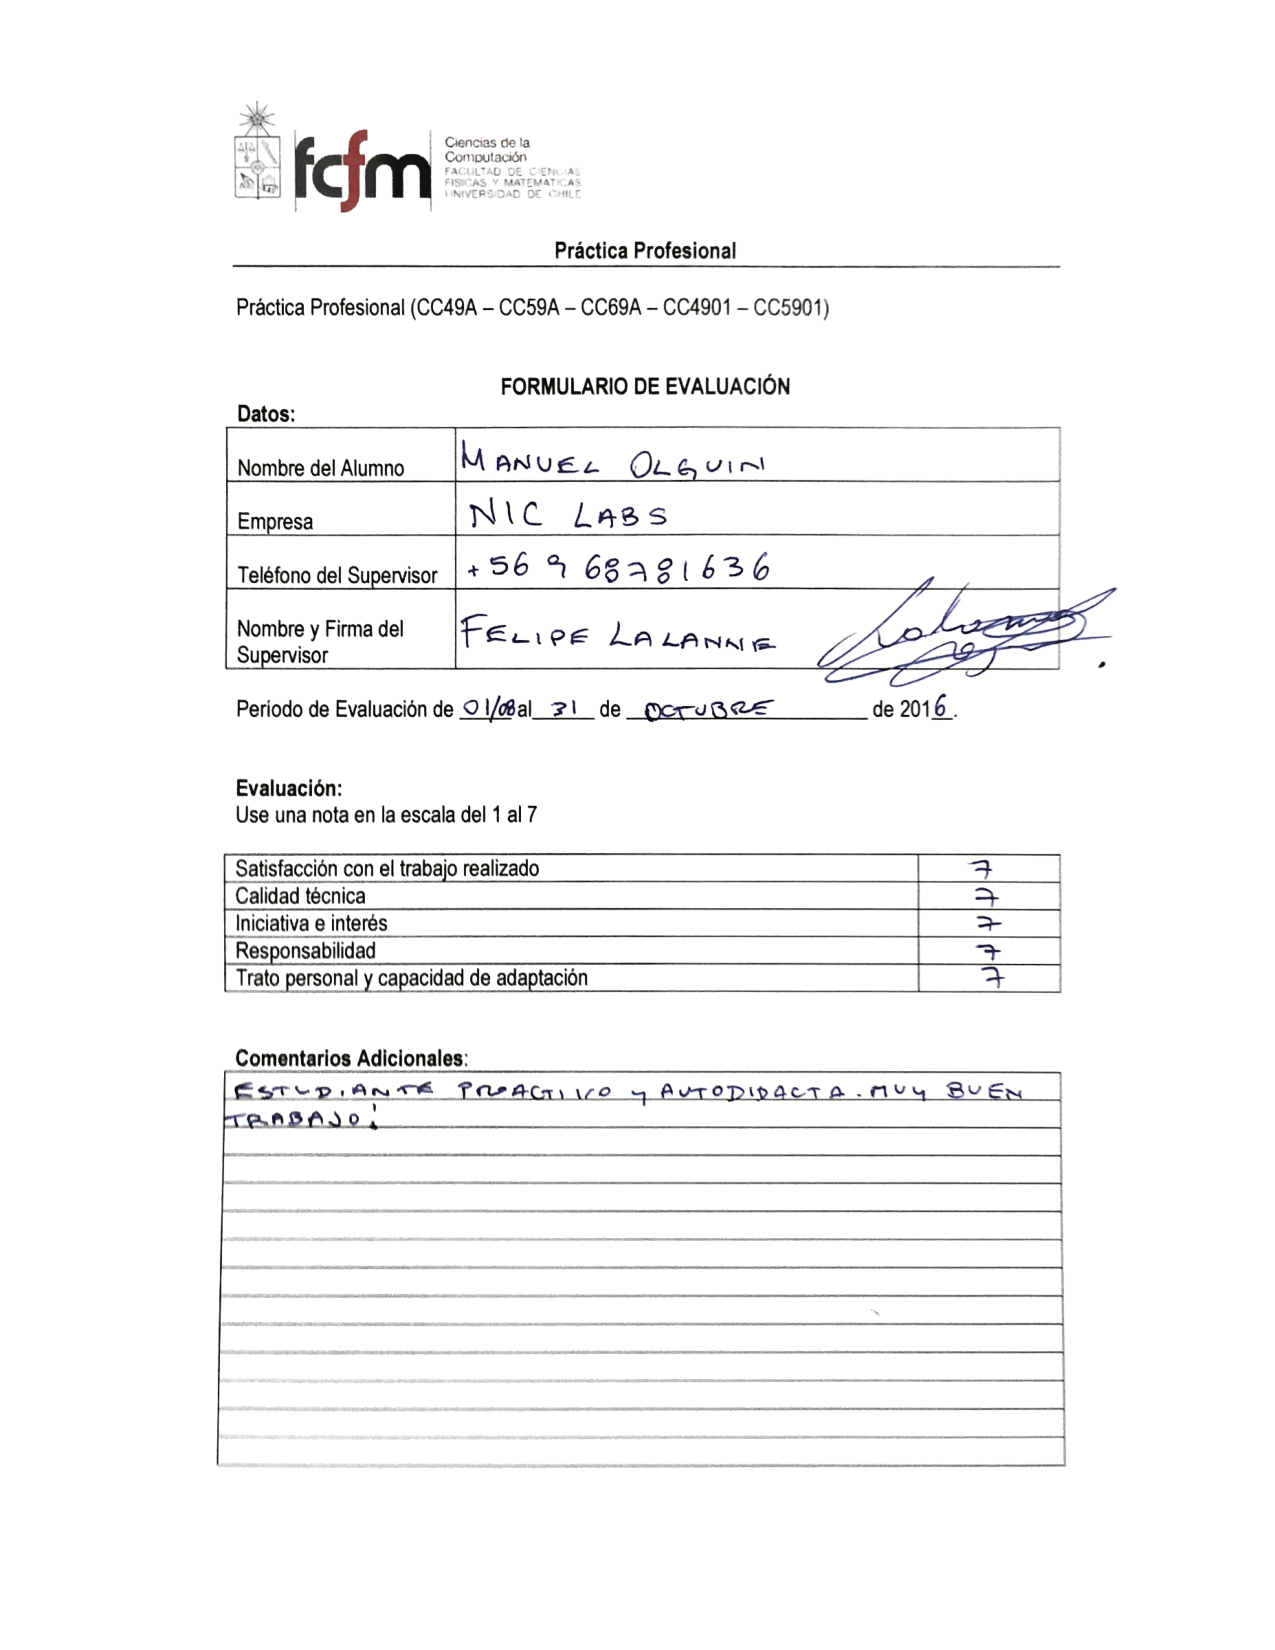
\includepdf{evaluacion/evaluacion.pdf}
\newpage
\section{Observaciones}
\newpage
% =============== INDICE ===============

\tableofcontents
%\listoffigures

% =============== SECCION ===============
\newpage
\section{Resumen}

El trabajo se realizó entre Agosto y Octubre del 2015 en NIC Chile Research Labs, el laboratorio de investigación y desarrollo en protocolos de internet de la Facultad de Ciencias Físicas y Matemáticas de la Universidad de Chile. \@ Consistió en
\begin{enumerate}
    \item rediseñar y actualizar parte de la API del backend de BeCity, una aplicación Android desarrollada en el laboratorio, para que se adhiriera al modelo REST.
    \item diseñar e implementar un microservicio de manejo de imágenes para el proyecto SUR.
\end{enumerate}

BeCity es una aplicación móvil Android orientada a ciclistas, la cual pretende facilitar el tránsito del usuario por la ciudad. Cuenta con un servicio de búsqueda de rutas con ciclovías, y permite grabar los recorridos del usuario, guardando estadísticas de velocidad, distancia recorrida, calorías quemadas y otros datos relevantes. Funciona bajo el paradigna cliente-servidor: existe un servicio central (el backend) que almacena y maneja los datos, y la aplicación Android (el cliente) se comunica con este servicio para actualizar y obtener información. Esta comunicación se realiza mediante una API (Application Programming Interface) usando HTTP (HyperText Transfer Protocol), sobre la cual se realizó el trabajo previamente mencionado.\\

El rediseño de esta API tenía como fin su modernización y adaptación a estándares modernos, en específico el modelo REST (REpresentational State Transfer)\\

SUR (Southern URban observatory) es una plataforma que pretende centralizar todos los proyectos desarrollados en NIC Chile Research Labs. En este sentido, SUR se plantea como un backend unificado para los distintos servicios, ofreciendo funcionalidades comunes como autentificación de usuarios y manejo de recursos como imágenes, y generando una integración más estrecha entre los servicios.\\

El trabajo realizado en SUR consistió en el diseño y posterior implementación de un pequeño servidor de imágenes, capaz de administrar recursos gráficos de manera eficiente, escalable y simple. Dicho servicio se encuentra actualmente estable y funcionando en la plataforma SUR.
\newpage
\section{Introducción}
\subsection{Lugar de Trabajo}

NIC Chile Research Labs (en adelante, NICLabs)\cite{niclabs}, es el laboratorio de redes de la Facultad de Ciencias Físicas y Matemáticas de la Universidad de Chile. Fundado en 2007, sus principales áreas de investigación y desarrollo son protocolos de internet y seguridad informática.

El trabajo detallado en el presente informe se desarrolló entre octubre y diciembre del año 2015, de manera presencial en las instalaciones del laboratorio ubicadas en Av. Blanco Encalada 1975, Santiago, Chile.

\subsection{Equipo de Trabajo}

%Arreglar!%

NICLabs cuenta tanto con desarrolladores e investigadores de tiempo completo, así como con estudiantes de pre- y postgrado. En específico, el trabajo se desarrolló en una sala compartida con otras 6 personas de distintas especialidades (diseñadores, ingenieros y estudiantes de pregrado).

En cuanto a los proyectos descritos en el presente informe, ambos se desarrollaron bajo la dirección de Felipe Lalanne\cite{lalanne}, investigador y desarrollador experimentado del laboratorio. Cabe destacar que si bien existe un equipo de trabajo formalmente conformado para BeCity, éste sólo maneja y actualiza la versión actual del software, y por ende el practicante no se unió directamente a éste, ya que su trabajo consideraba el rediseño completo del backend.
Por otro lado, no existe grupo de trabajo para SUR, y el practicante trabajó directamente bajo la tutela del supervisor.
\newpage
\subsection{Software y Conceptos Importantes}
En términos generales, ambos proyectos se desarrollaron en el lenguaje de programación Python\cite{python}, utilizando además JetBrains Pycharm 5 Professional Edition\cite{pycharm} como IDE (\emph{Integrated Development Environment} - Entorno de Desarrollo Integrado) principal.

\subsubsection{REST}

El modelo REST\cite{rest} (por sus siglas en inglés, ``Representational State Transfer'') es una serie de restricciones arquitecturales que, aplicadas a un servicio web, inducen una serie de propiedades deseables (e.g. escalabilidad, estabilidad, rendimiento, etc). Al estar relacionado sólamente con la estructura arquitectural del software, no especifica detalles de implementación, y es independiente del lenguage de programación escogido.\\

A continuación, se expondrán brevemente las restricciones impuestas por el modelo REST:
\begin{enumerate}
    \item \textbf{Modelo Cliente - Servidor} \@ Debe existir una clara separación de responsabilidades mediante una interfaz uniforme. Por ejemplo, el servidor debe encargarse del almacenamiento y procesamiento de los datos, pero no de la representación visual de éstos, y vice-versa en el caso del cliente.
    \item \textbf{\textit{Statelessness} - Ausencia de Estados} \@ El servidor no debe guardar información del estado del cliente entre solicitudes. El estado es almacenado por el cliente; cada solicitud debe ser independiente y contener toda la información necesaria para realizarse.
    \item \textbf{Caché} \@ El servidor debe poder guardar solicitudes en caché para poder responder futuras solicitudes de manera más expedita.
    \item \textbf{Transparencia de Capas} \@ El cliente no debe poder determinar si está conectado directamente al servidor o a un servicio intermedio (proxy, etc).
    \item \textbf{Uniformidad de la Interfaz} \@ A su vez puede separarse en:
    \begin{itemize}
        \item \emph{Separación de recursos y su representación} \@ La representación externa de los recursos (datos) debe ser independiente de como son almacenados por el servidor. A su vez, estas representaciones contienen toda la información necesaria para poder modificar el recurso original.
        \item \emph{Identificación Uniforme de Recursos} \@ Por ejemplo, mediante URI's\cite{uri}.
        \item \emph{Mensajes Autodescriptivos} \@ Cada mensaje incluye información de cómo procesarse.
    \end{itemize}
\end{enumerate}

\subsubsection{API}

Una API\cite{api} (Application Programming Interface), en el contexto de servicios web, es una interfaz de interacción entre los componentes de un modelo servidor-cliente. Específicamente en el caso de una API RESTful, consiste en un conjunto de puntos de enlace (o, cómo se les referirá en el presente informe, \emph{``vistas''}) públicos en el servidor, a través de los cuales un cliente puede comunicarse e interactuar con el servicio central, utilizando verbos estándar de HTTP\cite{http} (\texttt{GET}, \texttt{PUT}, \texttt{POST} y \texttt{DELETE}).

% explicar rest + http + api?

\subsubsection{PostgreSQL}

PostgreSQL\cite{postgres} es una de las principales implementaciones modernas del lenguaje SQL (Structured Query Language - Lenguaje Estructurado de Consultas) para bases de datos. Es un sistema de base de datos relacional ampliamente utilizado en la industria, y en específico, en BeCity se ocupa para el almacenamiento y consulta de los datos proporcionados por los usuarios.

\subsubsection{Python}

Python es un lenguaje de programación interpretado, dinámico y de alto nivel, con énfasis en la fácil lectura de su código y su brevedad sintáctica. Es un lenguaje multipropósito, apto para programas de pequeña y gran escala, y con soporte para múltiples paradigmas de programación (orientado a objetos, funcional, imperativo y demases).

En el contexto del trabajo realizado, Python, principalmente en su versión 2.7 (aunque en algunas instancias se ocupó también la versión más nueva del lenguaje, 3.5), fue el lenguaje escogido para el desarrollo de los servicios. Esto, ya que debido a su popularidad, cuenta con una gran cantidad de librerías bien documentadas y mantenidas que facilitaron el desarrollo.

\subsubsection{JSON}

JSON\cite{json} (JavaScript Object Notation), es un estándar abierto de codificación de datos para la comunicación entre servidor y cliente, en la cual los datos se codifican en pares atributo-valor en ``cleartext'' (es decir, texto legible por humanos).
Por ejemplo, el siguiente extracto ilustra una posible codificación de la FCFM en JSON:
\begin{lstlisting}[language=JSON]
{
    "Nombre": "Facultad de Ciencias Fisicas y Matematicas",
    "Universidad": "Universidad de Chile",
    "Direccion": {
        "Calle": "Beauchef",
        "Numero": 850,
        "Comuna": "Santiago",
        "Region": "Metropolitana",
        "Pais": "CHILE"
    }
}
\end{lstlisting}

\subsubsection{Redis}

Redis\cite{redis} puede describirse como un ``almacén de estructuras de datos en disco'', y se utiliza comúnmente como base de datos y transmisor de mensajes; además, en conjunto con la librería \emph{Python RQ}\cite{rqworker} de Python, se puede utilizar como una cola de ejecución de tareas. Éste fue el uso que se le dió en el servidor de imágenes, para ejecutar ciertas tareas de tiempo de ejecución más largo de manera diferida.

%\subsubsection{Docker}
\subsubsection{BeCity}

BeCity es una aplicación para smartphones con el sistema operativo Android, la cual tiene como fin la recolección de datos de ciclistas (por ejemplo, recorridos populares en una ciudad o comuna). Además, ayuda a los usuarios a transitar de manera segura por la ciudad, ofreciendo rutas con ciclovías e información atingente.

\subsubsection{SUR - Southern Urban Observatory}

SUR es pretende ser un servicio de uso interno de INRIA Chile y NICLabs; una plataforma centralizada para todos los proyectos de ambos laboratorios. Pretende unificar de ésta manera muchos servicios que se encuentran replicados en los distintos proyectos (por ejemplo, manejo de usuarios) bajo una misma platforma, intengrando así de manera mucho más eficiente distintos proyectos y servicios otorgados por los laboratorios.

\subsection{Situación Previa}
\subsubsection{BeCity}

En agosto del 2015, BeCity como aplicación ya se encontraba en funcionamiento, siendo distribuída a través de la tienda de aplicaciones de Google, la ``Play Store'', y con su backend montado en el servidor de NICLabs. Sin embargo, si bien contaba con una API completa para la comunicación entre clientes y backend, ésta no seguía el estándar REST para servicios web, principalmente en lo que se refiere a la uniformidad de la interfaz y la transparencia de capas, además de no seguir el estándar HTTP (e.g. todas las solicitudes ocupaban el verbo POST independiente de si creaban o no recursos nuevos en el servidor). Dadas estas condiciones, se había decidido reconstruirla desde cero siguiendo rigurosamente el modelo REST, para asegurar su futura escalabilidad y estabilidad.

\subsubsection{SUR}

Cuando el practicamente comenzó su trabajo en NICLabs, SUR como proyecto sólo existía como idea. Prácticamente todo el trabajo desarrollado por el practicante para este proyecto fue desde cero.

\pagebreak
\subsection{Descripción General del Trabajo}

\subsubsection{BeCity}

El practicante diseñó e implementó parte de la nueva API, en específico el módulo de manejo de usuarios (con la excepción del sistema de autentificación, el cual fue implementado por Felipe Lalanne), siguiendo las restricciones del modelo REST para servicios web. El trabajo realizado se puede dividir en dos etapas:
\begin{enumerate}
    \item \emph{Diseño y Documentación} \\ En esta etapa, el practicante estudió la API existente del módulo escogido para entender el funcionamiento interno de éste, y los métodos que presentaba su interfaz. Luego, se diseñó y documentó la nueva versión del módulo, con especial énfasis en la nueva interfaz.
    \item \emph{Implementación y Testeo} \\ Luego de diseñado y documentado el módulo, se procedió a la implementación de las funcionalidades en código. Se utilizó el proceso de desarrollo ``Test Driven Development'', es decir, primero se escribían tests para funcionalidades deseadas, y luego se implementaban.
\end{enumerate}

\subsubsection{SUR}

El trabajo realizado en SUR consistió en el desarrollo de un servicio de manejo de imágenes centralizado para todos los proyectos de la plataforma. El servicio debía básicamente almacenar y servir imágenes proporcionadas por los proyectos, por ejemplo para avatares de usuario. Se requería especial énfasis en la modularidad del servicio, de tal manera de que pudiese interactuar con cualquier otro proyecto que se adhiriera a la plataforma SUR en el futuro.

El trabajo consistió de dos etapas:
\begin{enumerate}
    \item \emph{Diseño del Servicio}\\ Para comenzar, se determinaron los requerimientos del servicio; las funcionalidades deseadas y la manera de interactuar con éste. Además, se establecieron los detalles de la integración del servicio con el resto de SUR.
    \item \emph{Implementación y Testing}\\ Ya establecidos los requerimientos, se implementó el sistema deseado, empleando una estrategia de desarrollo iterativo basado en tests.
\end{enumerate}

\newpage
\section{Trabajo Realizado}

\subsection{BeCity}

BeCity tiene como fin el facilitar el tránsito del ciclista por la ciudad, a la vez que recopila información y estadísticas útiles proporcionadas por los mismos usuarios. Por lo tanto, el manejo de usuarios de una manera eficiente es fundamental para el funcionamiento del servicio, y por consiguiente éste fue el primer módulo de funcionalidad en ser rediseñado para la nueva versión del backend.

\subsubsection{Análisis de implementación anterior}

El primer paso en el rediseño del módulo de usuarios del backend de BeCity, fue el estudio y análisis de la implementación anterior. Esto con el fin de identificar funcionalidades claves que debían mantenerse o mejorarse en la nueva iteración del sistema.\\
Esta etapa se desarrolló al mismo tiempo que el practicante investigó de manera más profunda sobre el modelo REST y aprendió sobre el uso de las herramientas disponibles en Python para el desarrollo de sistemas de ésta índole.\\



\paragraph{Almacenamiento de la información de los usuarios\\\\}

El almacenamiento de los datos de usuario estaba implementado utilizando una base de datos PostgreSQL.
En el modelo de la base de datos, la información atingente a los perfiles de usuarios se dividía en dos tablas:

\begin{itemize}
    \item \emph{users} -- La cual almacenaba las propiedades fundamentales de los usuarios; email, contraseña, ID.
    \item \emph{profile} -- Donde se almacenaban los detalles adicionales del perfil del usuario, como su nombre real, fecha de nacimiento, y estadísticas varias.
\end{itemize}

Además existían tres tablas más, utilizadas para la autentificación y el inicio de sesión de los usuarios.\\

En términos de código, la interacción entre el servidor y la base de datos se realizaba a través de las abstracciones proporcionadas por las librerías de Python SQLAlchemy y Flask-SQLAlchemy. Éstas permiten definir las tablas de la base de datos como clases de Python, y la creación de una nueva entrada se reduce simplemente a la creación de una nueva instancia del objeto definido por dicha clase.\\
Las tablas anteriormente mencionadas estaban entonces implementadas mediante dos clases de Python muy simples:
\begin{itemize}
    \item \emph{User}, la cual simplemente contenía variables de instancia y un constructor que inicializaba los valores del email y la contraseña.
    \item \emph{Profile}, la cual a su vez almacenaba los datos del perfil de usuario, y contenía un método para pasar esta información a un formato JSON.
\end{itemize}
\newpage
\paragraph{API\\\\}

La API anterior de BeCity utilizaba la librería Flask de Python, la cual abstrae la implementación de los \emph{endpoints} como ``funciones de vista'' -- funciones de python asociadas a un URL específico. Bajo este paradigma, la antigua API de BeCity consistía en una colección de funciones sin ninguna coherencia arquitectural. No existía un formato de respuesta común, ni una manera de agrupar semánticamente las funciones asociadas a un mismo recurso. \\

Por otro lado, la implementación violaba el estándar HTTP y el modelo REST utilizando el verbo POST para todas las solicitudes, ya fuesen solicitudes de creación de recursos, o de eliminación de éstos. Ésto tenía la consecuencia adicional de que, en vez de asignar URL's por recursos, y disponer de múltiples operaciones distintas por URL dependiendo del verbo HTTP utilizado en las solicitudes, en la antigua API existían URL's asociados a \emph{operaciones}.

Para ilustrar los problemas anteriores: existía por ejemplo el \emph{endpoint} \texttt{/api/user/delete}, el cual sólo aceptaba el verbo HTTP POST, el cual recibía una ID de usuario en un mensaje JSON y lo eliminaba de la base de datos. Ésto, en una API conforme al modelo REST y sin violaciones del protocolo HTTP, se implementaría mediante un endpoint \emph{/api/users/\textless id\textgreater} (\emph{id} es variable), el cual entre otros, admite el verbo HTTP DELETE y elimina el usuario identificado por \emph{\textless id\textgreater}.\\

Finalmente, existía también una separación innecesaria de los accesos a los usuarios propiamente tal y sus perfiles, con endpoints distintos para cada uno (\texttt{/api/user} y \texttt{/api/profile} respectivamente).

\newpage
\subsubsection{Diseño de nueva implementación}

A partir de análisis anterior, el practicante pudo elaborar un nuevo diseño para el backend, completamente en línea con los requerimientos del modelo REST. Este diseño se detalla a continuación, junto con justificaciones de las deciciones tomadas.

\paragraph{Almacenamiento de la información de los usuarios\\\\}
Se decidió continuar utilizando PostgreSQL para el almacenamiento de datos, por las ventajas que presenta para el almacenamiento de la información que maneja BeCity. La información manejada por el sistema es inherentemente relacional, puesto que se trata de datos de usuarios y estadísticas que se relacionan mutuamente.\\

En términos del modelo de la base de datos, la información de los usuarios se subdividió en tres tablas:
\begin{enumerate}
    \item Tabla \emph{users}: Esta tabla almacena los datos fundamentales para la autentificación del usuario: su email, nombre de usuario y contraseña, esta última almacenada como un hash SHA256. Además, contiene relaciones con las dos otras tablas.
    \item Tabla \emph{user\_details}: Contiene los detalles no escenciales (desde el punto de vista de la autenficación) del usuario, como por ejemplo su nombre real y fecha de nacimiento.
    \item Tabla \emph{user\_stats}: Esta es una tabla especial que agrupa llaves foráneas a otra tabla, \emph{samples}. Cada entrada en esta última corresponde a una estadística almacenada (\emph{samples} por ejemplo almacena el último valor agregado, el máximo, el promedio, etc), por lo que cada llave foránea almacenada en \emph{user\_stats} corresponde a una entrada en \emph{samples}.
\end{enumerate}

Se determinó ésta subdivisión de la información con el fin de modularizar elementos individuales - de esta manera, por ejemplo, es posible modificar cómo se almacenan las estadísticas de cada usuario sin afectar su información de inicio de sesión. Además, la abstracción de las estadísticas en muestras almacenadas en una tabla aparte, hacen que en el futuro agregar nuevas métricas al sistema sea simple y directo - basta con agregar una nueva llave foránea a \emph{samples} en \emph{user\_stats}.

\paragraph{API\\\\}

La interacción entre clientes y servidor obedece al paradigma \emph{CRUD} (Create, Read, Update, Delete - crear, leer, actualizar y eliminar), por lo que la API asociada al módulo debía permitir por lo menos este reducido conjunto de operaciones. Considerando lo anterior, se definieron los siguientes puntos de enlace para la API:

\begin{enumerate}
    \item \texttt{/api/v1/users/} -- Corresponde al punto de acceso a la colección de usuarios, y admite los siguientes verbos HTTP:
    \begin{itemize}
        \item POST: Correspondiente a la operación \emph{Create} del modelo \emph{CRUD}, permite la creación de nuevos usuarios en el sistema (sólo disponible para administradores). Recibe los datos del usuario, lo crea, y luego retorna la ID del recurso creado.
        \item GET: Corresponde a la operación \emph{Read}, y permite obtener la lista de usuarios del sistema. Sólo disponible para administradores.
    \end{itemize}
    \newpage
    \item \texttt{/api/v1/users/\textless id\textgreater} -- Donde \textless id\textgreater \@ corresponde a una ID de usuario sobre el cual operar. Permite:
    \begin{itemize}
        \item GET: \emph{Read}, pero a diferencia del método mencionado anteriormente permite el acceso a los detalles de un usuario en específico, y es accesible por administradores y el usuario mismo.
        \item PUT: \emph{Update}, permite la actualización de los datos de un usuario. Disponible para administradores y el usuario mismo.
        \item DELETE: \emph{Delete}, para eliminar un usuario por completo. Sólo accesible por administradores.
    \end{itemize}
    \item \texttt{/api/v1/users/stats/\textless id\textgreater} -- Permite acceder a las estadísticas de un usuario específico:
    \begin{itemize}
        \item PUT: Actualiza las estadísticas del usuario.
        \item GET: Retorna el detalle de las estadísticas.
    \end{itemize}
\end{enumerate}

Se determinó además que todo intercambio de información entre servidor y cliente (y viceversa), debiese hacerse a través de mensajes en formato JSON. Esto ya que dicho formato permite mantener la estructura lógica y las relaciones internas de los datos al pasarlos a una representación textual, y además agrega menos \emph{overhead} que otros lenguajes de \emph{markup}, como por ejemplo XML.\\

Además, para evitar ciertos problemas de seguridad que existen al retornar listas de objetos JSON directamente en los mensajes, se dictaminó el encapsulamiento de todos los mensajes que originan desde el servidor en un ``sobre'' JSON adicional:

\begin{lstlisting}[language=json, title=Ejemplo de ``sobre'' JSON.]
{
    'ok': True,
    'result': <resultado de la operacion>
}
\end{lstlisting}

\subsubsection{Implementación}

Como se mencionó anteriormente, la implementación se llevó a cabo utilizando Python 2.7, en parte por su amplio repertorio de librerías. Entre las librerías utilizadas, podemos destacar:
\begin{itemize}
    \item Flask\cite{flask}, la cual proporciona un framework básico para el desarrollo de aplicaciones web en Python. Por ejemplo, simplifica la ejecución de una aplicación Python como un servicio web asíncrono, y provee abstracciones para la implementación de endpoints (URL's) para interactuar con la aplicación.
    \item SQLAlchemy\cite{sqlalchemy} (junto con su extensión Flask-SQLAlchemy\cite{flasksqlalchemy}), para la interacción con la base de datos PostgreSQL. Provee abstracciones para la fácil definición de tablas y sus relaciones a través de clases en Python.
    \item Restless\cite{restless}, librería que proporciona una capa de abstracción para la creación de endpoints de servicios web como clases de Python.
\end{itemize}

\paragraph{Modelo Base de Datos\\\\}

El modelo de la base de datos se implementó utilizando las abstracciones de SQLAlchemy, definiendo clases de Python para cada una de las tablas antes mencionadas. Éstas cuentan con constructores que se encargan de inicializar las entradas con información por defecto, y con métodos para modificar los datos que aseguran sus consistencia interna.\\

Por ejemplo, a continuación se muestra el modelo de la tabla \emph{user\_details}:
\begin{lstlisting}[title=Modelo de la tabla \emph{user\_details}]
class UserDetails(db.Model):
    __tablename__ = 'user_details'

    id = db.Column(db.Integer, primary_key=True)
    created = db.Column(db.DateTime, default=now)
    modified = db.Column(db.DateTime, default=now, onupdate=now)

    name = db.Column(db.String(100))
    description = db.Column(db.Text)
    birth_date = db.Column(db.DateTime, default=datetime.strptime('19900101', '%Y%m%d'))
    gender = db.Column(ChoiceType(Genders), default=Genders.O)
    cyclist = db.Column(ChoiceType(CyclistTypes), default=CyclistTypes.ACR)

    # TODO: Implement image handler
    image = db.Column(db.String)

    user_id = db.Column(db.Integer, db.ForeignKey('users.id'), nullable=False)

    def __init__(self,
                 user,
                 name='',
                 description='',
                 birth_date=None,
                 gender=None,
                 cyclist=None,
                 image=''):

        self.user_id = user.id

        self.name = name
        self.description = description

        if birth_date is not None:
            self.birth_date = birth_date
        if gender is not None:
            self.gender = gender
        if cyclist is not None:
            self.cyclist = cyclist

        # TODO: image handler
        self.image = image
\end{lstlisting}

Las columnas de la tabla se definen como variables internas de la clase, y en este caso es posible evidenciar 10 columnas distinas: id, created, modified, name, description, birth\_date, gender, cyclist, image y user\_id. Se incluye también un constructor que se encarga de inicializar las columnas, verificando que datos requeridos no queden en blanco. Entonces, para crear una nueva entrada en la tabla basta con crear una nueva instancia de la clase \texttt{UserDetails}, y luego confirmar su creación en la base de datos utilizando \texttt{db.session.add()} y \texttt{db.session.commit()}, métodos incluídos en SQLAlchemy.\\

La tabla \emph{users} se define de manera similar, mientras que por otro lado, \emph{user\_stats} y \emph{samples} tienen consideraciones especiales que se verán a continuación.\\

\begin{lstlisting}[title=Modelo de la tabla \emph{samples}]
class Sample (db.Model):
    __tablename__ = 'samples'
    id = db.Column(db.Integer, primary_key=True)
    created = db.Column(db.DateTime, default=now)
    modified = db.Column(db.DateTime, default=now, onupdate=now)

    max = db.Column(db.Float, default=0.0)
    min = db.Column(db.Float, default=0.0)
    var = db.Column(db.Float, default=0.0)
    std = db.Column(db.Float, default=0.0)  # standard deviation
    mean = db.Column(db.Float, default=0.0)
    current = db.Column(db.Float, default=0.0)

    _sum = db.Column(db.Float, default=0.0)
    _sumsqr = db.Column(db.Float, default=0.0)  # for calculating E(X^2) -> used for the variance
    size = db.Column(db.Float, default=0.0)

    def update(self, sample):

        self.size += 1
        self._sum += sample
        self._sumsqr += math.pow(sample, 2)

        self.current = sample

        self.max = sample if sample >= self.max or self.max == 0 else self.max
        self.min = sample if sample <= self.min or self.min == 0 else self.max

        self.mean = (self._sum / self.size)
        self.var = (self._sumsqr / self.size) - math.pow(self.mean, 2)  # var = E(X2) - (E(X))2
        self.std = math.sqrt(self.var)
\end{lstlisting}

Como se comentó anteriormente, \emph{samples} almacena muestras estadísticas: cada entrada en la tabla corresponde a una estadística (ya sea peso, distancia, etc) de algún usuario. Como tales, las entradas no debiesen ser modificadas directamente, sino que se utiliza un método  \texttt{update()} que actualiza la estadística, recalculando por ejemplo el promedio y la varianza cada vez que se agrega una nueva muestra.\\
\newpage
Por otro lado, el modelo de la tabla \emph{user\_stats}, se ve como sigue (extracto):
\begin{lstlisting}[title=Modelo de la tabla \emph{user\_stats} (extracto)]
class UserStats(db.Model):
    __tablename__ = 'user_stats'
    id = db.Column(db.Integer, primary_key=True)
    created = db.Column(db.DateTime, default=now)
    modified = db.Column(db.DateTime, default=now, onupdate=now)

    user_id = db.Column(db.Integer, db.ForeignKey('users.id'), nullable=False)

    speed_id = db.Column(db.Integer, db.ForeignKey('samples.id'), nullable=False)
    distance_id = db.Column(db.Integer, db.ForeignKey('samples.id'), nullable=False)
    calories_id = db.Column(db.Integer, db.ForeignKey('samples.id'), nullable=False)
    weight_id = db.Column(db.Integer, db.ForeignKey('samples.id'), nullable=False)

    def __init__(self):
        speed = Sample()
        distance = Sample()
        calories = Sample()
        weight = Sample()

        db.session.add(speed)
        db.session.add(distance)
        db.session.add(calories)
        db.session.add(weight)
        db.session.commit()

        self.speed_id = speed.id
        self.distance_id = distance.id
        self.calories_id = calories.id
        self.weight_id = weight.id
\end{lstlisting}

Cada una de las columnas (excepto id, created y modified) corresponden a llaves foráneas a entradas en \emph{samples}, las cuales contienen información sobre las muestras estadísticas de éste usuario en específico. A su vez, cuenta con un método especial para actualizar (y mostrar) las muestras de una manera que mantenga la consistencia del sistema.
\pagebreak
\begin{lstlisting}[title=Rutina de actualización de muestras estadísticas.]
    def update_stats(self, speed=None, distance=None, calories=None, weight=None):

        sample_speed = Sample.query.filter(Sample.id == self.speed_id).first()
        sample_distance = Sample.query.filter(Sample.id == self.distance_id).first()
        sample_calories = Sample.query.filter(Sample.id == self.calories_id).first()
        sample_weight = Sample.query.filter(Sample.id == self.weight_id).first()

        change = False

        if speed is not None:
            sample_speed.update(speed)
            change = True
        if distance is not None:
            sample_distance.update(distance)
            change = True
        if calories is not None:
            sample_calories.update(calories)
            change = True
        if weight is not None:
            sample_weight.update(weight)
            change = True
        if change:
            db.session.commit()

        return sample_speed, sample_distance, sample_calories, sample_weight
\end{lstlisting}

\paragraph{API\\\\}

Se utilizó la librería Restless, junto con un wrapper escrito previamente por Felipe Lalanne, para la abstracción de la creación de endpoints de la API. Los recursos se modelaron como clases de Python, con métodos específos para las operaciones \emph{CRUD}.\\

Se definieron dos clases para el manejo de las vistas: la clase \texttt{UserResource}, la cual maneja el acceso a los detalles de usuario, y la clase \texttt{UserStatsResource}, cuyo fin es manejar el acceso a las estadísticas de usuario.

\subparagraph{UserResource:\\} Esta clase abstrae los puntos de acceso para el manejo de datos no estadísticos de los usuarios, y su estructura general es:
\begin{lstlisting}
@api.resource('/api/v1/users/')
class UserResource:

    @api.grant(Roles.ADMIN)
    def list(self):
        ...

    # /api/v1/users/<pk>/
    @api.grant(Roles.ADMIN, Roles.USER)
    def detail(self, pk):
        ...

    @api.grant(Roles.ADMIN)
    def create(self):
        ...

    @api.grant(Roles.ADMIN, Roles.USER)
    def update(self, pk):
        ...

    @api.grant(Roles.ADMIN)
    def delete(self, pk):
        ...
\end{lstlisting}

La clase está registrada en el endpoint \texttt{/api/v1/users/}, y contiene métodos para cada una de las operaciones \emph{CRUD}, tanto para la colección completa, como para usuarios específicos. Por ejemplo, el método \texttt{detail()} de la clase es el encargado de retornar detalles sobre usuarios específicos:
\begin{lstlisting}[title=Método de obtención de detalles de usuario.]
# /api/v1/users/<pk>/
@api.grant(Roles.ADMIN, Roles.USER)
def detail(self, pk):
    if Grant.check_grant(self.user, Roles.ADMIN):
        user = User.query.filter(User.username == pk).first()
        return {
            'id': user.username,
            'created': user.created.isoformat(),
            'modified': user.details.modified.isoformat(),
            'email': user.email,
            'name': user.details.name,
            'description': user.details.description,
            'birth_date': user.details.birth_date.isoformat(),
            'gender': user.details.gender,
            'cyclist': user.details.cyclist,
            'image': user.details.image
        }

    if self.user.username == pk:
        return {
            'id': self.user.username,
            'created': self.user.created.isoformat(),
            'modified': self.user.details.modified.isoformat(),
            'email': self.user.email,
            'name': self.user.details.name,
            'description': self.user.details.description,
            'birth_date': self.user.details.birth_date.isoformat(),
            'gender': self.user.details.gender,
            'cyclist': self.user.details.cyclist,
            'image': self.user.details.image
        }

    raise Unauthorized('Only admins and data owners can view user data')
\end{lstlisting}
\newpage
Cabe destacar que toda transferencia de información entre servidor y cliente se hace en formato JSON, de manera de mantener la estructura lógica de la información transferida. En el ejemplo anterior, el servidor al ser consultado por los detalles de un usuario en específico, responde con un objeto JSON que contiene la información deseada (además de información del resultado de la operación):
\begin{lstlisting}[language=json, title=Ejemplo de respuesta del servidor.]
{
    'ok': True,
    'result': {
        'id': '067e61623b6f4ae2a1712470b63dff00',
        'created': '1970-01-01T00:00:01.000001',
        'modified': '1970-01-01T00:00:01.000010',
        'email': 'foo@bar.baz',
        'name': 'Foo Bar',
        'description': 'Lorem ipsum dolor sit amet.',
        'birth_date': '1970-01-01T00:00:01.000001',
        'gender': 'M',
        'cyclist': 'ACR',
        'image': ''
    }
}
\end{lstlisting}

Por otro lado, la comunicación de cliente a servidor sigue un formato parecido. Tomando por ejemplo, el método \texttt{create()}, encargado de la creación de nuevos usuarios, expuesto a continuación (extracto). Este método obtiene la información del usuario a crear desde el cliente en un objecto JSON idéntico al objeto retornado en el campo \texttt{`result'} del JSON retornado por \texttt{detail()} (con la adición del campo \texttt{`password'}).
\begin{lstlisting}[title=Extracto del método de creación de usuarios.]
def create(self):
    ...

    user = User(
        email=self.data.get('email'),
        password=self.data.get('password')
    )

    # Always create details
    gender = self.data.get('gender', None)
    if gender and gender not in Genders:
        raise BadRequest(("Gender must be one of (" + ','.join(["'%s'"] * len(Genders)) + ")") % tuple(Genders))
    cyclist = self.data.get('cyclist', None)
    if cyclist and cyclist not in CyclistTypes:
        raise BadRequest(("Gender must be one of (" + ','.join(["'%s'"] * len(Genders)) + ")") % tuple(Genders))

    try:
        bdate = datetime.strptime(self.data.get('birth_date', '1990-01-01'), '%Y-%m-%d')
    except ValueError:
        raise BadRequest(
            'Birth date must be in ISO-8601 format, only including year, month and day. Example: 1990-01-01')

    user.details = UserDetails(user=user,
                               name=self.data.get('name', None),
                               description=self.data.get('description', ''),
                               birth_date=bdate,
                               gender=gender,
                               cyclist=cyclist,
                               image=self.data.get('image', '')
                               )

    # Always init stats:
    user.stats = UserStats()
    db.session.add(user)

    ...

    db.session.commit()

    return {
            'id': user.username,
            'created': user.created.isoformat(),
            ...
        }
\end{lstlisting}
\begin{lstlisting}[language=json, title=Ejemplo de datos para solicitud de creación de usuario.]
{
    'email': 'foo@bar.baz',
    'password': 'foobarbaz'
    'name': 'Foo Bar',
    'description': 'Lorem ipsum dolor sit amet.',
    'birth_date': '1970-01-01',
    'gender': 'M',
    'cyclist': 'ACR',
}
\end{lstlisting}
\pagebreak
\subparagraph{UserStatsResource:\\}

Por su parte, esta clase está asociada al conjunto de \emph{endpoints} \texttt{/api/v1/users/stats/\textless id\textgreater}, y sólo posee métodos para la consulta y actualización de estadísticas de usuarios individuales (no de la colección completa, ya que no tiene sentido). En específico, posee dos métodos -- uno para la consulta de las estadísticas de un usuario dado, y otra para la modificación de éstas. La implementación de éstas es relativamente simple: el método de consulta simplemente busca las estadísticas en la base de datos, las empaca en un diccionario JSON y las retorna. Por otro lado, el método de modificación recibe una solicitud con las muestras a ingresar en un JSON, las desempaca y las agrega a la base de datos.\\

\begin{lstlisting}[title=Extracto del método de consulta de estadísticas de usuario.]
# /api/v1/users/stats/<pk>/
@api.grant(Roles.ADMIN, Roles.USER)
def detail(self, pk):
    ...

    speed, distance, calories, weight = userstats.get_stats()

    return {
        'user': userstats.user.username,
        'weight': {
            'max': weight.max,
            'min': weight.min,
            'current': weight.current
        },
        'speed': {
            'max': speed.max,
            'min': speed.min,
            'average': speed.mean
        },
        'calories': {
            'max': calories.max,
            'min': calories.min,
            'average': calories.mean
        },
        'distance': {
            'max': distance.max,
            'min': distance.min,
            'average': distance.mean
        }
    }
\end{lstlisting}

\newpage
\subsection{SUR}

Como se ha mencionado anteriormente, el proyecto SUR pretende ser una plataforma central para todos los proyectos de INRIA Chile y NICLabs - con el fin de centralizar varios servicios que actualmente se encuentran ``duplicados'' en los proyectos (por ejemplo, manejo de usuarios y de imágenes). Un servicio central como SUR permitiría que cierta información se pudiese compartir de manera transparente entre los proyectos y servicios, permitiedo por ejemplo que usuarios usen sus mismas credenciales de inicio de sesión, evitando la redundancia de tener que crear cuentas en cada uno de los servicios.\\

La plataforma en sí está diseñada como un conjunto de microservicios individuales, cada uno con una labor específica y acotada, que se presentan al cliente como una API única y coherente. Los servicios deben entonces ser relativamente independientes, pero a la vez poder comunicarse y coordinarse entre sí.

% % ················ IMAGEN ·················
\begin{figure}[ht!]
\centering
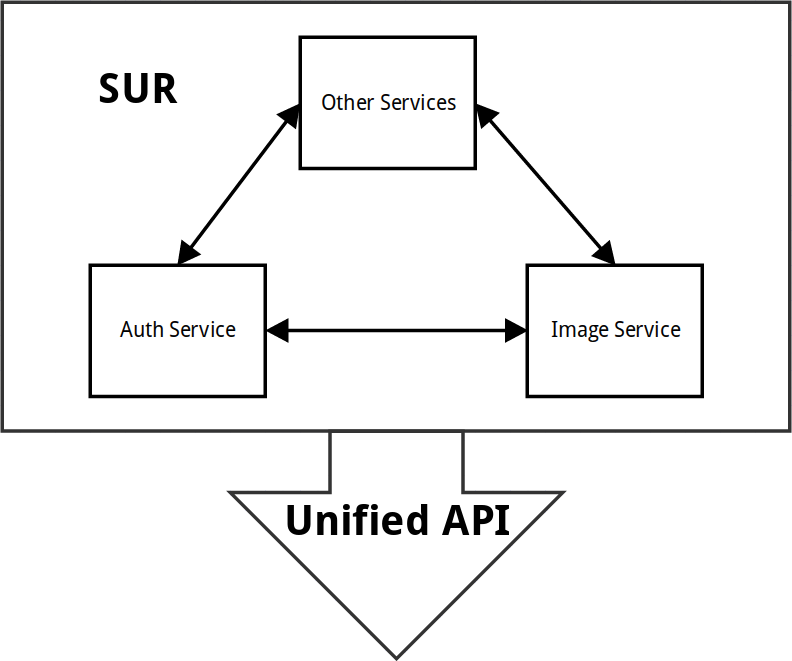
\includegraphics[scale=0.5]{img/diagrama_SUR.png}
\caption{Diagrama arquitectural de SUR}\label{sur}
\end{figure}
% %··········································


Bajo esta lógica fue que al practicante se le solicitó la implementación del servicio central de imágenes, el cual permitiese compartir de manera transparente y eficiente recursos de imágenes (por ejemplo, avatares de usuario) entre los proyectos. Este servicio debía además interactuar con el servicio de autentificación de usuarios (desarrollado en paralelo por Felipe Lalanne), para restringir el acceso a las imágenes almacenadas.
\pagebreak
\subsubsection{Especificaciones}

El servicio en cuestión debía seguir una serie de especificaciones generales que aseguraban su eficiencia, escalabilidad y su compatibilidad con los demás servicios de la plataforma.

\begin{enumerate}
    \item \emph{Independencia} -- \@ La implementación del servicio de imágenes debía ser independiente y agnóstica de la implementación del resto de los servicios. Es decir, si bien podía exister interdependencia entre el servicio de imágenes, y (por ejemplo) el servicio de autentificación, ésta no podía depender de la implementación de cada uno. Esto para asegurar que en el futuro, los servicios pudiesen actualizarse o cambiarse completamente sin perturbar el resto de los servicios en la plataforma.
    \item \emph{Adherencia al modelo REST} -- \@ El servicio debía basarse en el paradigma cliente-servidor, y seguir las especificaciones del modelo REST; comunicación mediante verbos HTTP, no almacenar estados, etc.
    \item \emph{Simplicidad} -- \@ El código debía ser simple y conciso, y no agregar demasiada complejidad al sistema.
    \item \emph{Instántaniedad} -- \@ Finalmente, la respuesta del servicio a solicitudes por parte de clientes debiese ser expedita, y no causar esperas prolongadas.
\end{enumerate}

Además, se establecieron una serie de requerimientos funcionales de los servicios que debía proveer el sistema:
\begin{enumerate}
    \item Almacenamiento de imágenes. Por simplicidad, sólo se debía aceptar imágenes en el formato \emph{Portable Network Graphics}, \textbf{.png}.
    \item Descarga de imágenes del servidor, en tamaños y resoluciones no necesariamente iguales a las originales.
    \item Eliminacion de imágenes almacenadas.
\end{enumerate}
\newpage
\subsubsection{Diseño Arquitectural}

En concordancia con las especificaciones y requerimientos anteriores, se llegó al diseño arquitectural detallado en esta sección.\\

El lenguaje escogido para la implementación fue nuevamente Python 2.7, principalmente por su amplio repertorio de librerías para desarrollo web, además de su simplicidad y elegancia sintáctica. Adicionalmente, es el lenguaje en el que están escritos todos los demás servicios de SUR, asegurando así una coherencia arquitectural interna de la plataforma.\\

Entre las librerías del lenguaje que fueron utilizadas, podemos destacar:
\begin{itemize}
    \item Flask\cite{flask}, para el desarrollo de la base de la aplicación web.
    \item Pillow\cite{pillow}, librería de manejo de imágenes. Provee métodos de alteración de imágenes (transformaciones de tamaño, formato, etc).
\end{itemize}

Por otro lado, se descartó utilizar una base de datos para el servicio, ya que toda la información de las imágenes se puede manejar a través de \emph{metadatos} y almacenarse en el sistema de archivos. Agregar un sistema de bases de datos aumentaría la complejidad del sistema de manera innecesaria.\\

Finalmente, para poder asegurar la rapidez del servicio, se decidió realizar ciertas solicitudes de manera diferida -- esto es, no se ejecutan inmediatamente, sino que quedan en una cola de solicitudes y eventualmente se resuelven. Esto se implementó para solicitudes por parte de clientes que no requieren una respuesta inmediata del servidor y que además son intensas en términos de tiempo de ejecución (por ejemplo, la carga de una nueva imagen al servicio, ya que ésta operación requiere además un procesamiento posterior). Se efectuó mediante el uso de un servidor Redis en conjunto con el servicio de imágenes, el cual almacena y ejecuta las operaciones en la cola.
\newpage
\subsubsection{Implementación}

La implementación del código se llevó a cabo siguiendo una estrategia iterativa basada en tests, implementando funcionalidades básicas y asegurándose de su correcto funcionamiento mediante tests antes de pasar a funcionalidades más complejas.

\paragraph{1. Carga de imágenes al servidor}

Ésta fue la primera funcionalidad en implementarse en el servidor, dada que puede considerarse una de las dos funcionalidades fundamentales del servicio (la otra sería la descarga de imágenes).\\

Funciona de la siguiente manera: el servidor expone públicamente una vista (en este caso, ``/v1/images'') que acepta solicitudes HTTP con el verbo POST. Esta solicitud debe incluir los siguientes HEADERS:
\begin{verbatim}
    Content-Type: multipart/form-data
    Content-MD5: <checksum MD5 del archivo>
\end{verbatim}
Además, debe incluir el archivo a subir en formato binario en el cuerpo de la solicitud. \\

Al recibir la solicitud, el servidor primero ejecuta pruebas para verificar la existencia y validez de los datos proporcionados. En esta etapa el proceso puede arrojar tres variantes del mismo error HTTP ``400 Bad Request'', el cual se utiliza para notificar al cliente de que su solicitud no cumple con el formato requerido. En este caso, se lanza el error en caso de ausencia del archivo a cargar, o en caso de que la solicitud no incluya un HEADER con el hash MD5 de la imagen o que éste esté incorrecto.\\
Verificada la validez de la solicitud, el servidor pasa a almacenar y procesar la imagen (si la imagen ya existe en el sistema de archivos, el servidor simplemente retorna un mensaje HTTP ``201 Created''). En esta etapa también se verifica que el archivo cargado sea efectivamente una imagen, y el servidor retorna nuevamente un ``400 Bad Request'' de no ser así.\\

El procesamiento de las imágenes se hace de manera diferida - al terminar las verificaciones mencionadas previamente, el servidor guarda la imagen en disco y agrega un procedimiento a la cola de procesamiento del servidor Redis (además de retornar ``201 Created'' junto con el hash de la imagen al cliente). La rutina diferida de procesamiento ejecutada por el servidor Redis es la siguiente:
\pagebreak
\begin{lstlisting}
def process_image(filename):
    """
    Deferred image handling routine.
    Generates a set of images of various resolutions from an original image.
    :param filename: ID of the original image.
    :rtype: None
    """
    try:
        o_img = Image.open(UPLOAD_FOLDER + filename + '/original.png', 'r')
        o_img.save(UPLOAD_FOLDER + filename + '/original.png', format='png')
        resolutions = app.config['STD_RESOLUTIONS']

        for resolution in resolutions:
            n_img = o_img.copy()
            n_img.thumbnail(resolution, Image.ANTIALIAS)
            n_img.save('{0}{1}/{2}.png'.format(UPLOAD_FOLDER, filename, resolution[0], resolution[1]), format='png')
            n_img.close()

        o_img.close()
    except IOError:
        shutil.rmtree(UPLOAD_FOLDER + filename)
\end{lstlisting}


Para evitar manejar los nombres de las imágenes (por ejemplo, por consideraciones de seguridad), éstas se identifican mediante su hash MD5: al recibir una imagen nueva, el servidor crea un directorio en la carpeta de imágenes cuyo nombre es el hash de la imagen, y luego almacena la imagen recibida bajo el nombre ``original.png'' dentro de dicho directorio. Luego, la rutina diferida ``process\_image()'' se encarga de crear múltiples resoluciones de la misma imagen para su rápido acceso en el futuro, las cuales se almacenan bajo el mismo directorio mencionado anteriormente.\\

Finalmente, una imagen con hash MD5 \texttt{CB5DED429F491D8337FC58006468CF35} cargada correctamente al servidor quedaría almacenada de la siguiente manera:
\begin{verbatim}
UPLOAD_FOLDER/
    CB5DED429F491D8337FC58006468CF35/
        original.png
        48.png
        128.png
        256.png
        ...
\end{verbatim}

Donde los archivos \texttt{48.png}, \texttt{128.png}, etc., corresponden a resoluciones específicas precalculadas para su rápido acceso en el futuro.
\pagebreak
\paragraph{2. Descarga de imágenes}

La descarga de imágenes fue la segunda funcionalidad en implementarse, y funciona como se detalla a continuación.

Para descargar una imagen, el cliente debe conocer su ID (la cual corresponde al hash MD5 de la imagen). El servidor a su vez cuenta con una vista ``/v1/images/\textless image\_id\textgreater''; la notación \emph{\textless image\_id\textgreater} denota que esta parte del URL es variable - en específico, el cliente debe reemplazar \emph{\textless image\_id\textgreater} por la ID de la imagen que se solicita. Esta vista acepta los métodos GET y DELETE de HTTP (el verbo correspondiente a la solicitud de descarga es, evidentemente, el verbo GET), además de una serie de parámetros HTTP en el URL:
\begin{enumerate}
    \item tamaño precalculado: El cliente puede solicitar un tamaño precalculado de la imagen usando el parámetro \emph{``thumbnail=\textless thumb\_size\textgreater''} (de no existir, se creará).
    \item a escala: Utilizando el parámetro \emph{``scale=\textless scale\textgreater''}, se puede solicitar la imagen a cierta escala respecto al original.
    \item transformada: Finalmente, el cliente puede solicitar la transformación de la imagen mediante el uso de los parámetros \emph{``width=\textless w\textgreater''} y \emph{``height=\textless h\textgreater''} para especificar directamente el ancho y la altura de la imagen deseados, respectivamente.
\end{enumerate}

Por ejemplo, un cliente que desee obtener la imagen \texttt{CB5DED429F491D8337FC58006468CF35} transformada a \texttt{1280x720} (sin mantener la relación de aspecto), debería efectuar la siguiente solicitud:
\begin{center}
\texttt{GET /v1/images/CB5DED429F491D8337FC58006468CF35?width=1280}\&\texttt{height=720}
\end{center}


Internamente, las solicitudes son manejadas por el servidor de la siguiente manera:
primero, se verifica la existencia de la imagen, y de no existir se retorna un código de error ``404 Not Found'' al cliente.
Verificada ya la existencia de la imagen solicitada, se procede a servir la imagen de acuerdo a los parámetros solicitados por el cliente (si la solicitud no incluye parámetros, se retorna directamente la imagen original). De especial interés son aquellas solicitudes con el parámetro ``thumbnail'', ya que éstas son solicitudes para resoluciones populares y estándar de la imagen. Tienen el efecto de que, de no existir el tamaño solicitado, este es creado y almacenado por el servidor, de tal manera que futuras solicitudes para dicho tamaño sean más expeditas.\\

\begin{lstlisting}[title=Extracto de código encargado de manejar solicitudes de tamaños precalculados.]
# Thumbnail requests are done first, because they are faster
# System now checks if there is a precomputed size stored and sends that instead.
try:
    thumb = int(request.args.get('thumbnail', 0))
except ValueError:
    raise BadRequest400(error="Width, Height and Thumbnail must be Integers, Scale must be Float")
except TypeError:
    raise BadRequest400(error="Width, Height and Thumbnail must be Integers, Scale must be Float")

filename = UPLOAD_FOLDER + image_id + '/' + str(thumb) + '.png'

if thumb != 0 and os.path.exists(filename):  # if it exists, send it
    img = Image.open(filename)
    try:
        return send_image(img)
    except IOError:
        app.logger.error('Error when trying to send image ' + image_id)
        raise IOError

elif thumb != 0:  # if it doesn't, create and then send it
    img = img.copy()
    img.thumbnail((thumb, thumb), Image.ANTIALIAS)
    img.save(filename)

    try:
        return send_image(img)
    except IOError:
        app.logger.error('Error when trying to send image ' + image_id)
        raise IOError
\end{lstlisting}

Finalmente, se procesan las solicitudes con los parámetros de escala, ancho y alto, ya que estos requieren procesamiento en el lugar de la imagen, y demoran más.

\paragraph{3. Eliminación de imágenes}

La eliminación de imágenes se implementó mediante una rutina simple que recibe la ID de la imagen a eliminar y elimina completamente el directorio relacionada con dicha imagen.

\begin{lstlisting}
@auth.check_auth
def delete_image(image_id):
    """
    Deletes an image from the server.
    Requires auth, and only admins should be able to call this method.
    Note that this deletes the original image and ALL associated thumbnails.
    :param image_id: The ID of the image to be deleted.
    """
    if os.path.exists(UPLOAD_FOLDER + image_id):
        shutil.rmtree(UPLOAD_FOLDER + image_id)
        app.logger.info('Deleting image: ' + image_id)
        return create_body(result='Image deleted.'), 201
    else:
        raise NotFound404(error='Image with ID={0} not found.'.format(image_id))
\end{lstlisting}

\paragraph{4. Integración con servicio de Auth}

El servicio de autentificación de usuarios fue desarrollado en paralelo por Felipe Lalanne, y la integración entre ambos servicios fue el último paso en el desarrollo del servidor de imágenes. \\

La integración entre ambos servicios funciona de la siguiente manera:
\begin{enumerate}
    \item El servicio de Auth expone internamente un \emph{endpoint} que recibe un token de autentificación a validar en los parámetros del URL. Este \emph{endpoint} luego retorna un código HTTP 200 si el token es válido, y 404 si no.
    \item Por su parte, el servicio de imágenes implementa un \emph{wrapper} en torno a sus métodos que requieren autentificación, el cual extrae el token de las solicitudes entrantes y lo envía al servidor de autentificación para su validación. En caso de ser válido, se ejecuta el método solicitado, y en caso contrario retorna un código de error al cliente indicando que su autentificación no es válida.
\end{enumerate}
\pagebreak
En términos de implementación, el \emph{wrapper} encargado de la extracción y validación de los tokens es el siguiente:
\begin{lstlisting}
def check_auth(self, view):
    """
    Wraps a view function, and checks the authorization of each request on said view.
    :param view: The view to be protected by the auth service.
    """

    @wraps(view)
    def wrap_view(*args, **kwargs):

        if self.app.config.get('TESTING') or self.app.config.get('DEBUG'):
            # always return true if testing
            return view(*args, **kwargs)

        token = get_token_from_request()
        if token is not None:
            authenticated = self.check_token(token)
            if authenticated:
                return view(*args, **kwargs)
            else:
                raise Unauthorized401()
        else:
            raise Unauthorized401(error='missing_token', error_description='No authorization token provided.')

    return wrap_view
\end{lstlisting}
Este método simplemente verifica que el token sea válido, y de serlo, procede a la ejecución de la vista solicitada. Sin embargo, en caso de error de autentificación (ya sea token vencido o inexistente), envía en vez un código de error HTTP 401 Unauthorized al cliente.\\

Finalmente, el método encargado de la validación del token es relativamente simple -- básicamente, envía una solicitud al servidor de autentificación, incluyendo el token a validar como parámetro del URL, y retorna \emph{True} o \emph{False} si el token es válido o no, respectivamente.

\begin{lstlisting}
def check_token(self, token):
    """
    Sends a request to the auth service to verify the validity of a token.
    Returns a boolean indicating the validity (or not) of the token.
    :param token: String - the token to be validated.
    :return: Boolean - True if the token is valid, False otherwise.
    """
    if token is None:
        return False

    rv = requests.get(self.auth_url, params={'token': token})
    if rv.status_code == 404:
        return False

    return True
\end{lstlisting}

\newpage
\section{Conclusiones}

El trabajo descrito por el presente informe de práctica fue evaluado por el supervisor, Felipe Lalanne, y fue considerado como suficientemente satisfactorio como para incorporar al practicante al personal permanente de NICLabs.\\

Desgraciadamente, por razones internas, la continuación del proyecto de BeCity está actualmente en discusión dentro de la directiva del laboratorio. El trabajo efectuado por el practicante no ha sido entonces incluído en el código de producción, aunque conforma una sólida base para del desarrollo de una futura versión del proyecto.\\

Por otro lado, el proyecto SUR ha sido adoptado en su totalidad por INRIA Chile, fundación sin fines de lucro enfocada en la investigación y desarrollo en áreas de las ciencias de la computación, dónde se continúa su desarrollo. La implementación del servidor de imágenes fue evaluada como satisfactoria, y si bien presenta algunos \emph{bugs}, se considera lo suficientemente estable como para justificar su uso dentro del proyecto. \\

Dentro de la experiencia y el aprendizaje técnico obtenidos por el practicante durante el periodo, destacan:
\begin{itemize}
    \item La adquisición de conocimiento sobre tecnologías y estándares web, como el modelo REST y el desarrollo de backends y servicios en Python.
    \item La aplicación de las enseñanzas obtenidas en la carrera sobre bases de datos relacionales, y el aprendizaje práctico de cómo interactuar con éstas mediante lenguajes de alto nivel.
\end{itemize}

Finalmente, destaca también la experiencia adquirida en la aplicación práctica de la \emph{ingeniería de software}, y el trabajo en una empresa. Por ejemplo, se adquirío valioso conocimiento sobre las distintas etapas del desarrollo de software, desde el diseño inicial y la identificación de requerimientos, pasando por el desarrollo mismo y el testeo del software. Por otro lado, se aprendió a utilizar de manera correcta y eficiente herramientas de desarrollo colaborativo como lo son los sistemas de control de versión (en este caso, \emph{git}), y la correcta documentación de un software -- y en particular, la documentación de una API que en algún momento podría llegar a ser pública.
\newpage
%\section{Apéndices}
%\subsection{BeCity}
%\subsubsection{Modelo de Base de Datos}
%\lstinputlisting{code/becity_models.py}
%\newpage
%\subsubsection{Implementación de Vistas}
%\lstinputlisting{code/becity_views.py}
%\newpage
%\subsection{SUR}
%\subsubsection{Implementación de Vistas}
%\lstinputlisting{code/sur_views.py}
%\newpage
%\subsubsection{Integración con Servicio de Auth}
%\lstinputlisting{code/sur_auth.py}
%\newpage
\begin{thebibliography}{5}
    \bibitem{niclabs} \emph{NIC Chile Research Labs} - \url{http://niclabs.cl}

    \bibitem{lalanne} \emph{Felipe Lalanne} - \url{https://github.com/pipex}

    \bibitem{python} \emph{The Python Programming Language} - \url{https://www.python.org/}

    \bibitem{pycharm} \emph{JetBrains Pycharm} - \url{https://www.jetbrains.com/pycharm/}

    \bibitem{rest} \emph{RESTful Web Services} - \url{http://www.ibm.com/developerworks/library/ws-restful/}

    \bibitem{uri} \emph{URI - Uniform Resource Identifier}: cadena de caracteres utilizada para identificar recursos específicos, siguiendo un esquema definido.\\ \url{https://en.wikipedia.org/wiki/Uniform_Resource_Identifier}

    \bibitem{api} \emph{Application Programming Interface} - \url{https://en.wikipedia.org/wiki/Web_API}

    \bibitem{http} \emph{HyperText Transfer Protocol Verbs} - \url{https://www.w3.org/Protocols/rfc2616/rfc2616-sec9.html}

    \bibitem{postgres} \emph{PostgreSQL - ``The world's most advanced open source database.''}\\ \url{http://www.postgresql.org/}

    \bibitem{json} \emph{Javascript Object Notation} - \url{http://www.json.org/}

    \bibitem{redis} \emph{Redis} - \url{http://redis.io/}

    \bibitem{rqworker} \emph{Python RQ:} Library for Python background workers. - \url{http://python-rq.org/}

	\bibitem{flask} \emph{Flask is a microframework for Python based on Werkzeug, Jinja 2 and good intentions.}\\ \url{http://flask.pocoo.org/}

    \bibitem{restless} \emph{Restless - A lightweight REST miniframework for Python.}\\ \url{https://restless.readthedocs.org/en/latest/}

    \bibitem{sqlalchemy}\emph{SQLAlchemy - The Python SQL Toolkit and Object Relational Mapper}\\ \url{http://www.sqlalchemy.org/}

    \bibitem{pillow}\emph{PILLOW - Python Imaging Library fork}\\ \url{https://pillow.readthedocs.org/en/3.1.x/}
\end{thebibliography}

% ============= FIN DE DOCUMENTO ==============
\end{document}

% % ················ IMAGEN ·················
% \begin{figure}[ht!]
% \centering
% \fbox{\includegraphics[scale=0.6]{img/flujo.png}}
% \caption{Flujo de caja anual}\label{flujo}
% \end{figure}
% %··········································

% % ················ IMAGEN DOBLE ·················
% \begin{figure}[ht!] \centering
% \subfloat[Esquemático]{\includegraphics[scale=0.44]{img/seguidor.png}}
% \subfloat[Simulación]{\includegraphics[scale=0.45]{img/seguidor1.png}}
% \caption{Simulación como seguidor de voltaje}\label{seguidor}
% \end{figure}
% %··········································
